\chapter{System Description and Previous work}
\section{Description of System}
\subsection{Parts of the system}
\subsubsection{Qubits}
A qubit is a quantum bit, the analog in quantum computing to the binary digit or bit of classical computing. Just as a bit is the basic unit of information in a classical computer, a qubit is the basic unit of information in a quantum computer. \citep{Whatisqubit} 
%\textbf{cite whatis}
\par
In simple words, a qubit is a two level quantum mechanical system.
%\newline \textbf{\emph{fig3}}
\begin{figure}[h]
\centering
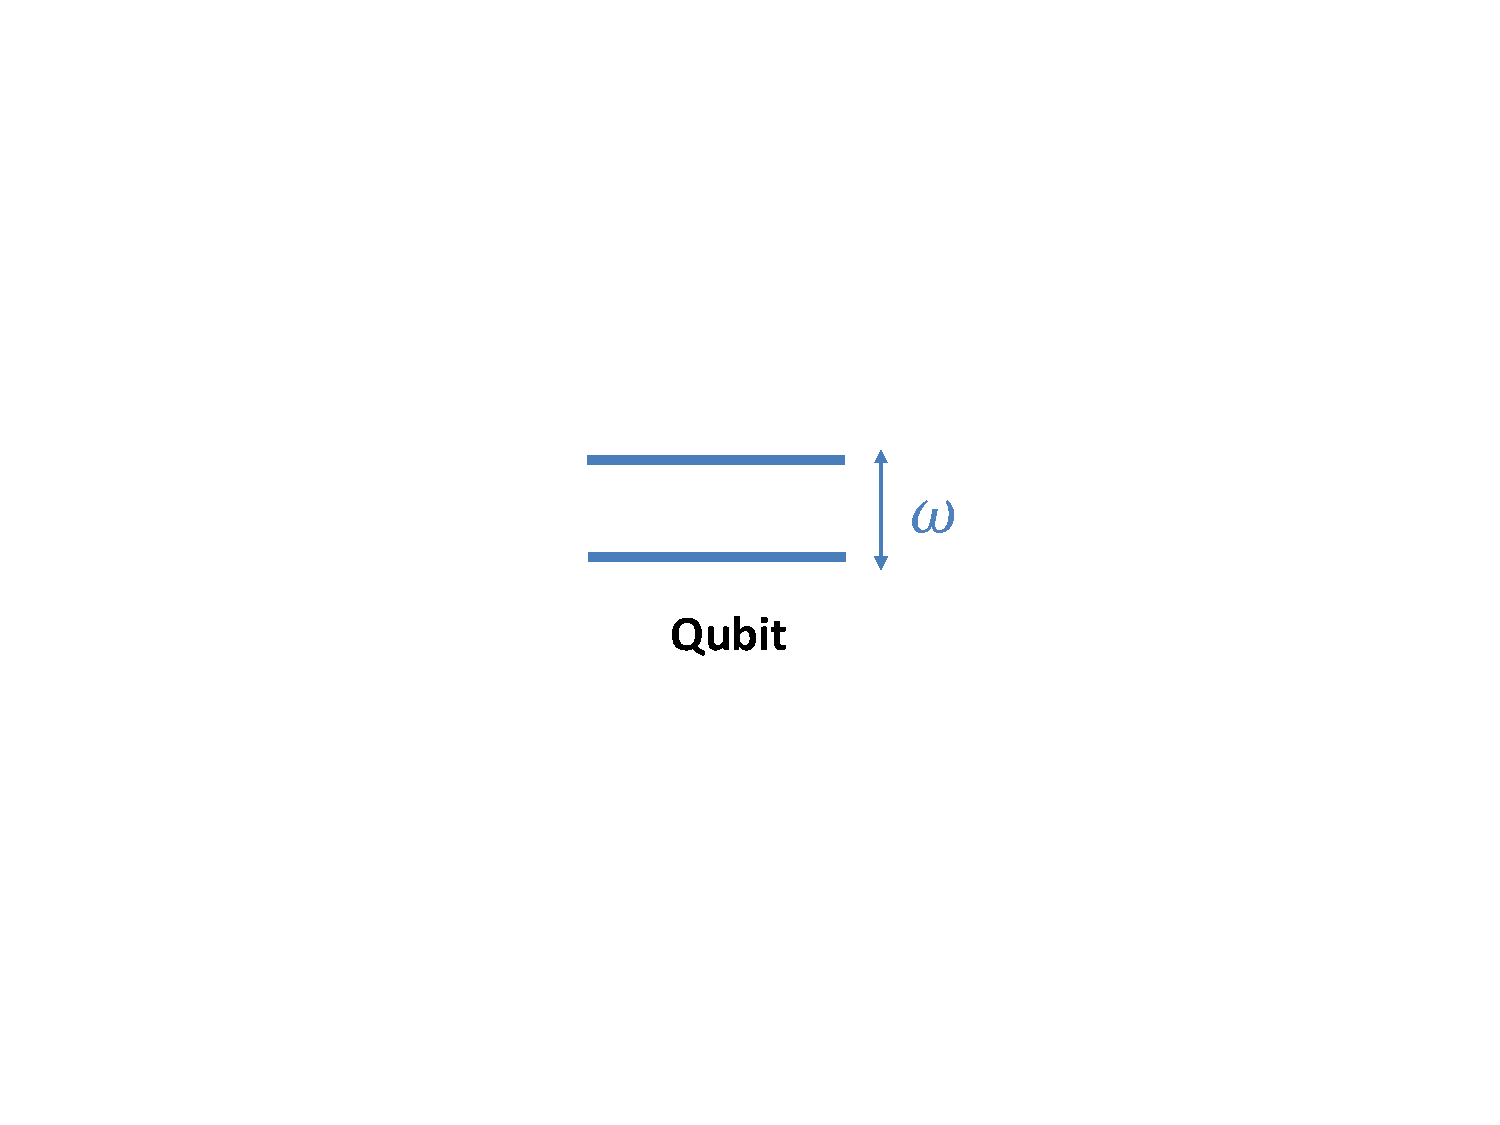
\includegraphics[width=0.5\textwidth]{Figr3a.pdf}
\caption{Qubit}
\label{fig:Figr3a}
\end{figure}


\subsubsection{Electromagnetic cavity}
An electromagnetic cavity  is an enclosure where standing electromagnetic waves can be sustained for considerable periods of time with or without an external driving field.%\citep{wiki:resonator}
%\textbf{ cite wiki resonator}
%\newline \emph{fig4}
\begin{figure}%[h]
\centering
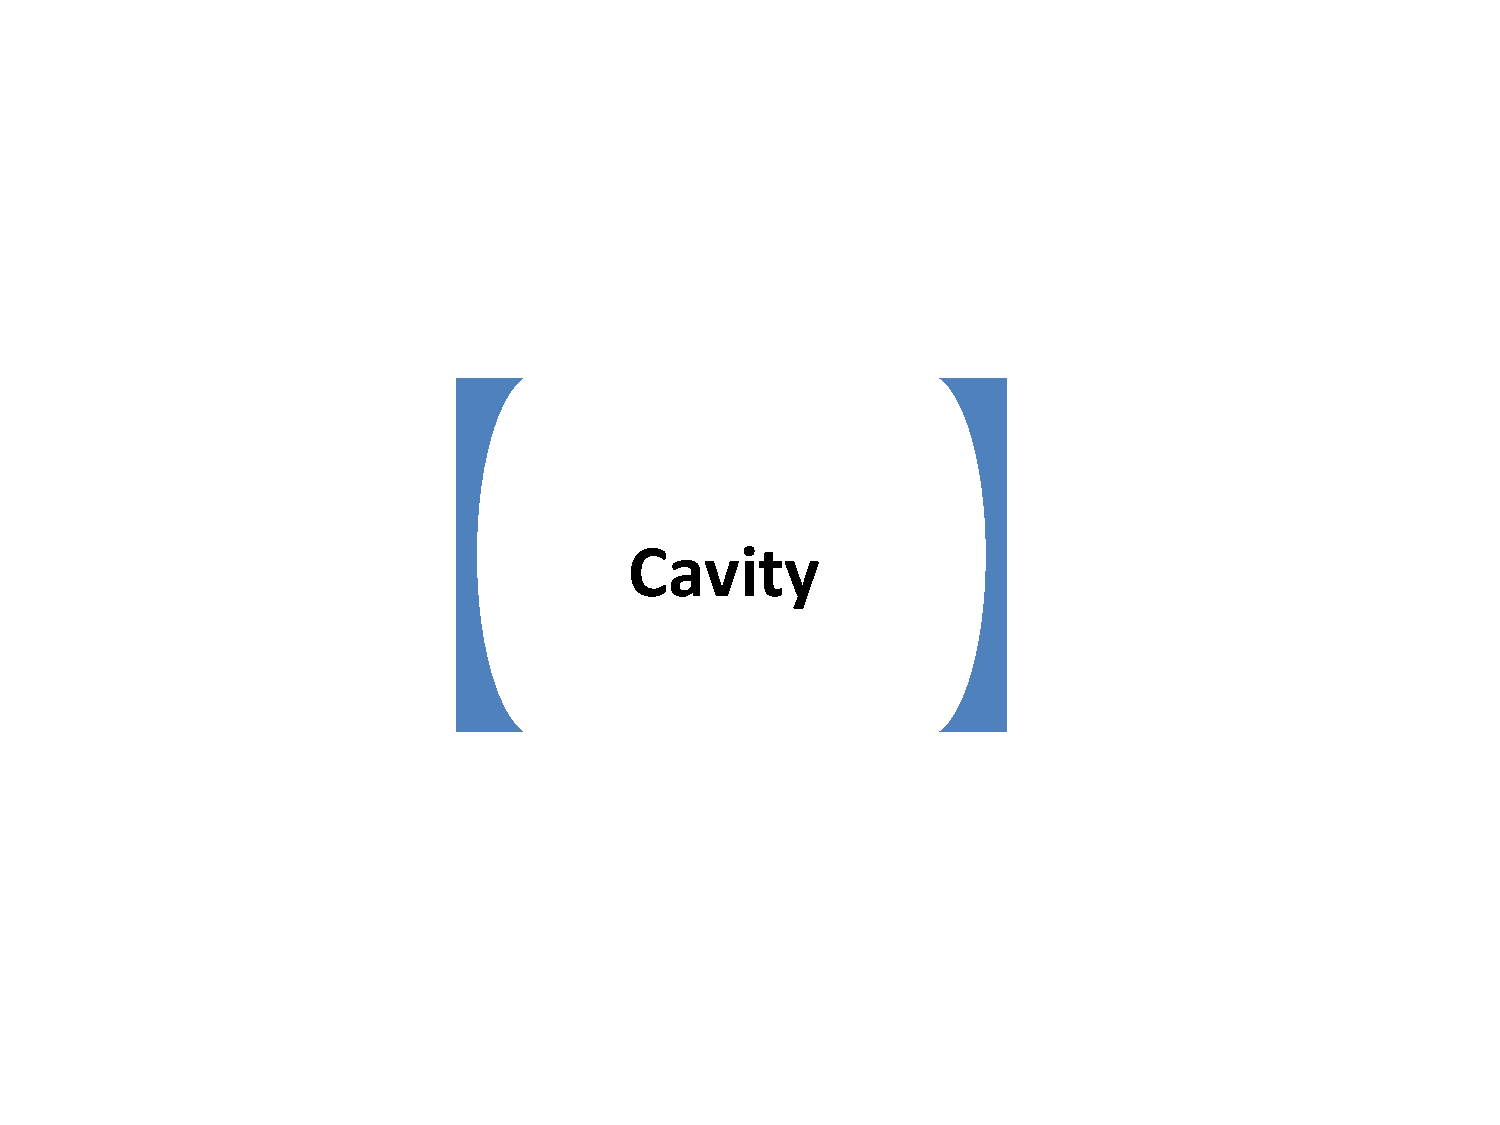
\includegraphics[width=0.5\textwidth]{Figr4a.pdf}
\caption{Cavity}
\label{fig:Figr4a}
\end{figure}

\subsubsection{Physics of system}
To exemplify how state transfer could be enhanced by tweaking the underlying Hamiltonian it would be better to do so by means of trying it out on an actual physical system. The physical system \citep{Tejas_APS1}  that we choose for this purpose is as follows : 
\begin{figure}[!h]
\centering
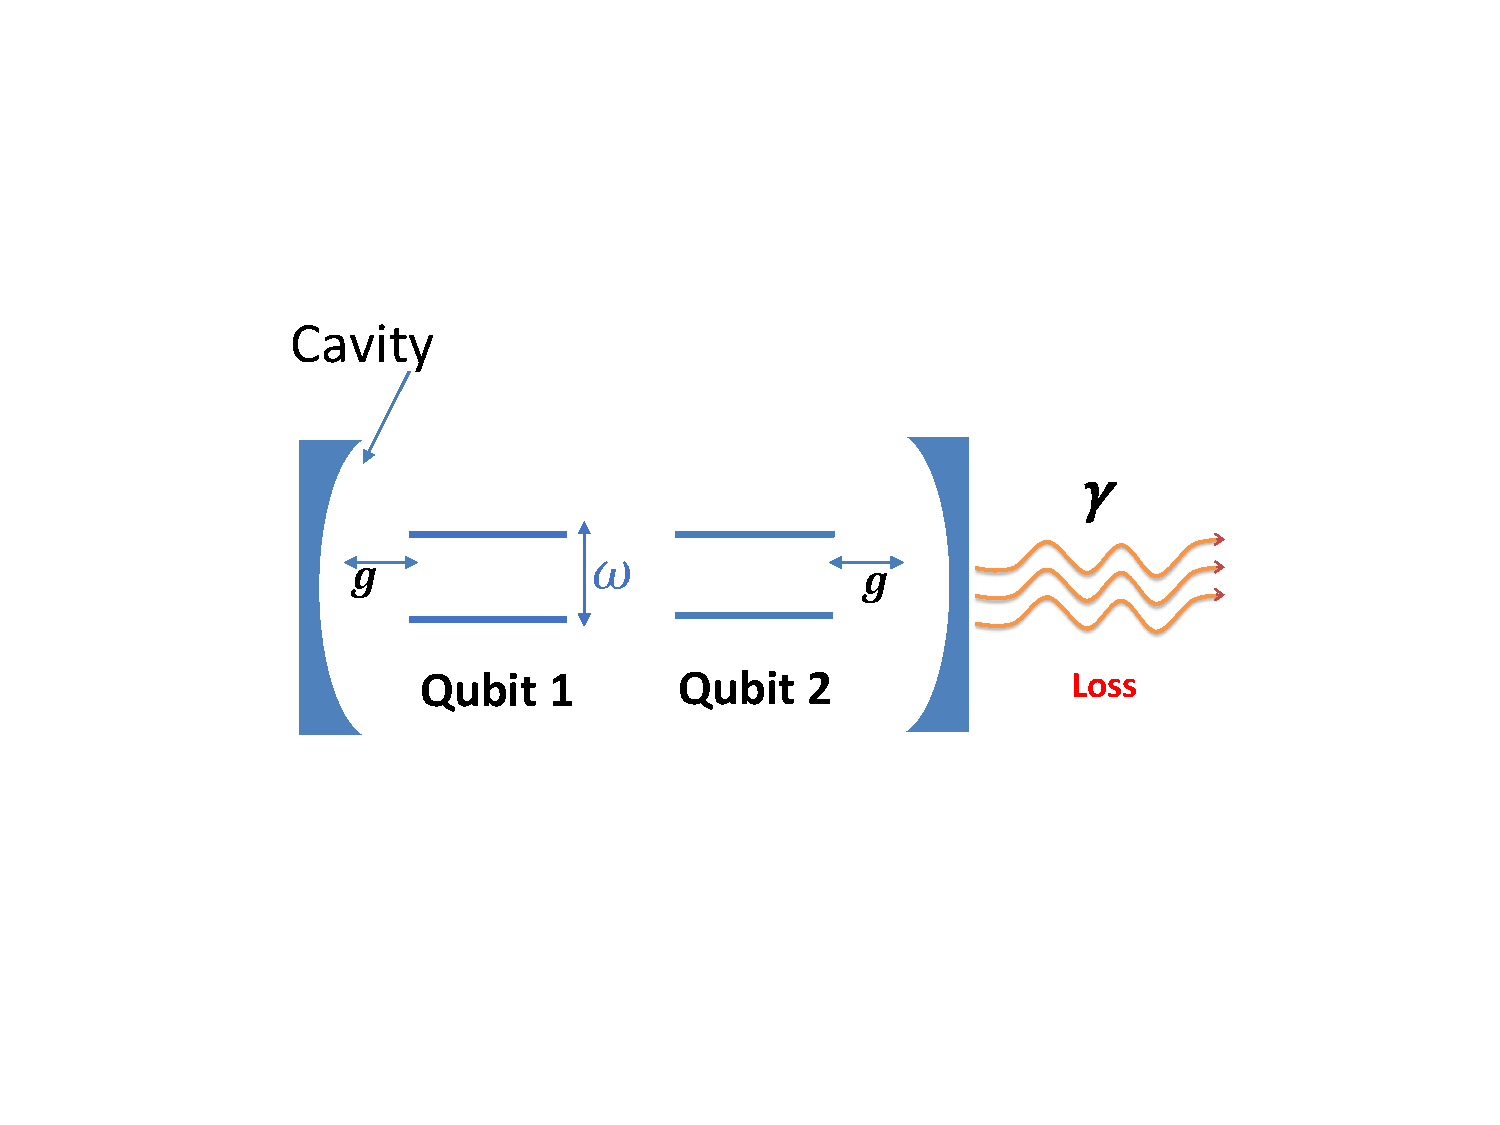
\includegraphics[width=0.8 \textwidth]{Figr1a.pdf}
\caption{Two qubits in a leaky cavity}
\label{fig:Figr1a}
\end{figure}


%The statement of the problem is as follows:
\begin{itemize}
\item We have:%\textbf{ cite my old aps }
\begin{enumerate}
\item Two qubits each with an energy difference of $(\hslash\thinspace{\omega})$.
\item A single mode lossy cavity approximated as a harmonic oscillator with energy spacing of $(\hslash\thinspace{\Omega})$.  
\end{enumerate}
\item Dissipation of quantum information occurs at a characteristic rate ($\gamma$).
\item There is no interaction between the qubits themselves.
\item Both the qubits are coupled to the cavity
\item The only way the qubits can communicate with each other is via the cavity
\end{itemize}

\subsection{Hamiltonian of the system}
The Hamiltonian of the system can be written as follows:
\begin{align}\label{eq:1}
H &= H_{0} + V
\end{align}
where $H_{0}$ is the bare Hamiltonian and $V$ is the coupling Hamiltonian. 
The bare Hamiltonian can be written as
\begin{align}\label{eq:2}
{H}_{0}&=\frac{\omega}{2}\thinspace{\sigma}_{z}\thinspace\otimes I^{(2)}\otimes{I^{(n)}}\thinspace + \thinspace\frac{\omega}{2}\thinspace{I^{(2)}}\thinspace\otimes\thinspace{\sigma}_{z}\otimes{I^{(n)}}\thinspace+\thinspace\Omega\thinspace I^{(2)}\otimes I^{(2)}\otimes{a}_{+}{a}_{- }
\end{align}
Where: 
\begin{itemize}
\item $\omega$ = frequency corresponding to the energy spacing  between the two levels of each qubit.
\item $\Omega$ = frequency corresponding to the difference in the energy levels of the cavity.
\item ${\sigma}_{z}, {\sigma}_{+}, {\sigma}_{-}$ =  Pauli matrices.   
\item ${a}_{+}, {a}_{-}$ = creation and annihilation operators for the cavity.
\item $I^{(2)}$ is the identity in the qubit Hilbert space.
\item $I^{(n)}$ is the identity in the harmonic oscillator Hilbert space.
\item $\hbar$ is set to be equal to $1$ in accordance with the usual practice. 
\end{itemize}
In the above equation~\eqref{eq:2} %\textbf{From2.2 }
\begin{itemize}
\item The first part represents bare Hamiltonian for the qubit 1.
\item The second part represents that of qubit 2.
\item The third  part represents that of  cavity. 
\end{itemize}

Now we will talk about how one would write down the interaction Hamiltonian $V$. Since, our system consists of qubits in a cavity effectively we have a double Jaynes Cummings type of Hamiltonian 
In our case since we have two qubits  we will have two couplings, \(g_{1}\) and \(g_{2}\). ${g}_{1}$ is the parameter related to the  strength of the coupling between the first qubit and the cavity. Similarly for ${g}_{2}$. So, following the discussion in the previous chapter we have 
\begin{align}\label{eq:15.1}
V &= V_{1} + V_{2}
\end{align}
Where: 
\begin{align}\label{eq 15.2}
V_{1}&= g_{1}\left({\sigma  }_{ - }\otimes I^{(2)}\otimes { a }_{ + }\thinspace + \thinspace{ \sigma }_{+}\otimes I^{(2)}\otimes{a}_{ - }\right)\\
V_{2}&= g_{ 2 }\left(I^{(2)}\otimes { \sigma  }_{ - }\otimes { a }_{ + }+I^{(2)}\otimes { \sigma  }_{ + }\otimes { a }_{ - }\right)
\end{align}


%\begin{itemize}
%\item $V_{1}= g_{1}\left({\sigma  }_{ - }\otimes I^{(2)}\otimes { a }_{ + }\thinspace + \thinspace{ \sigma }_{+}\otimes I^{(2)}\otimes{a}_{ - }\right)$
%\item $V_{2}= g_{ 2 }\left(I^{(2)}\otimes { \sigma  }_{ - }\otimes { a }_{ + }+I^{(2)}\otimes { \sigma  }_{ + }\otimes { a }_{ - }\right)$
%\end{itemize}

Putting all this together we get equation 
\begin{equation}\label{eq:16}
V= g_{1}\left({\sigma  }_{ - }\otimes I^{(2)}\otimes { a }_{ + }\thinspace + \thinspace{ \sigma }_{+}\otimes I^{(2)}\otimes{a}_{ - }\right)\thinspace
+\thinspace g_{ 2 }\left(I^{(2)}\otimes { \sigma  }_{ - }\otimes { a }_{ + }+I^{(2)}\otimes { \sigma  }_{ + }\otimes { a }_{ - }\right)
\end{equation}
Thus the full Hamiltonian is as follows:
\begin{multline}\label{FullH:1}
H =\frac{\omega}{2}\thinspace{\sigma}_{z}\thinspace\otimes I^{(2)}\otimes{I^{(n)}}\thinspace +\thinspace\frac{\omega}{2}\thinspace{I^{(2)}}\thinspace\otimes\thinspace{\sigma}_{z}\otimes{I^{(n)}}\thinspace+\thinspace\Omega\thinspace I^{(2)}\otimes I^{(2)}\otimes{a}_{+}{a}_{- } \\
+ g_{1}\left({\sigma  }_{ - }\otimes I^{(2)}\otimes { a }_{ + }\thinspace + \thinspace{ \sigma }_{+}\otimes I^{(2)}\otimes{a}_{ - }\right)\thinspace
+\thinspace g_{ 2 }\left(I^{(2)}\otimes { \sigma  }_{ - }\otimes { a }_{ + }+I^{(2)}\otimes { \sigma  }_{ + }\otimes { a }_{ - }\right)
\end{multline}
Where all the symbols are as defined earlier and $\hbar$ is set to be equal to $1$ in accordance with the usual practice.  
\subsubsection{Working of the system } 
This system works as follows:
\begin{itemize}
\item Qubit 1 is coupled to the cavity via the coupling Hamiltonian ${g}_{1}({\sigma  }_{ - }\otimes I^{(2)}\otimes { a }_{ + }\thinspace + \thinspace{ \sigma }_{+}\otimes I^{(2)}\otimes{a}_{ - })$. Through these coupling the state of qubit 1 is  being transferred to the cavity.
\item Similar to qubit 1, qubit 2 is also coupled via the coupling Hamiltonian ${g}_{2}\left(I^{(2)}\otimes { \sigma  }_{ - }\otimes { a }_{ + }+I^{(2)}\otimes { \sigma  }_{ + }\otimes { a }_{ - }\right)$. Through this coupling the information from the cavity is being transferred to qubit 2.
\item All this while the cavity is also leaking quantum information at a rate $\gamma$.
\end{itemize}

\subsection{Choice of Lindbladian operator}

Having derived the Lindblad equation in the previous chapter it is time to decide what would be the Lindbladian operators. One thing that we know is they must be of the same dimensions, shape etc. as that of the density matrix. This is because both of them live in the Hilbert space of the system.
\par 
We know that the cavity is a leaky one i.e. it undergoes spontaneous emissions. The cavity has been modelled as a harmonic oscillator. On undergoing emission the oscillator drops down from one fock state to the one below it. This is equivalent to the action of a annihilation operator acting on the harmonic space oscillator.
\par
Thus we can write 

\begin{align}\label{eq:1001}
L = I^{(2)} \otimes I^{(2)} \otimes {a}_{-}
\end{align}

where all the terms are the same as defined before 

\subsection{Putting it all together}
After all this hard work we end up with,

\begin{equation}\label{eq:1002}
\frac { {d\rho}_{s}}{dt} = -{ i\thinspace } [{ H },\thinspace { \rho  }_{ s }] +\gamma \left({ { L }\thinspace{ \rho}_{ s } }\thinspace { L }^{ \dagger  }-\frac { 1 }{ 2 } \{ { L }^{ \dagger}\thinspace{L},{\rho  }_{ s }\}\right)
\end{equation}

Where:
\begin{itemize}
\item $\rho_{s}$ = Density matrix for the system which includes both the qubits and the cavity.
\item  Total Hamiltonian as written in \eqref{FullH:1}\begin{multline}\notag
H =\frac{\omega}{2}\thinspace{\sigma}_{z}\thinspace\otimes I^{(2)}\otimes{I^{(n)}}\thinspace +\thinspace\frac{\omega}{2}\thinspace{I^{(2)}}\thinspace\otimes\thinspace{\sigma}_{z}\otimes{I^{(n)}}\thinspace+\thinspace\Omega\thinspace I^{(2)}\otimes I^{(2)}\otimes{a}_{+}{a}_{- } \\
+ g \left({\sigma  }_{ - }\otimes I^{(2)}\otimes { a }_{ + } + { \sigma }_{+}\otimes I^{(2)}\otimes{a}_{ - }
+ I^{(2)}\otimes { \sigma  }_{ - }\otimes { a }_{ + }+I^{(2)}\otimes { \sigma  }_{ + }\otimes { a }_{ - }\right)
\end{multline} where we have additionally set $g_{1}$ equal to $g_{2}$ and replaced both of them by $g$, since this is the case which we could consider while performing the numerical calculations. Here $g$ is the common coupling strength of the qubits to the cavity.
\item $ {L} = I^{(2)} \otimes I^{(2)} \otimes {a}_{-} $  Lindbladian operator as in \eqref{eq:1001}
\item $\gamma$ = Characteristic rate of dissipation for the cavity. 
\item $\hbar$ is set to be equal to $1$ in accordance with the usual practice. 
\end{itemize}


\section{Previous work}
The question that we wish to answer is that could we improve the state transfer by varying the coupling constant $g$ with time. In short, our aim is to see if one could enhance the fidelity to the target state if we make the coupling constant time dependent.   We tried to answer these questions by writing a code  in MATLAB \textsuperscript{\textregistered}.  This code uses the built in function fmincon (an interior point algorithm which minimizes functions using some gradient optimization techniques).
One may wonder why  use fmincon if one wants to maximize ? Doesn't fmincon contain the word "min" instead of "max". The trick is that we minimize the negative of the fidelity to determine the optimum pulse sequence for a piece wise constant $g(t)$.

In this chapter we present some of the results that we obtained by numerically solving the Lindblad equation \Eqref{eq:1002} in MATLAB\textsuperscript{\textregistered}.

We have undertaken a comparative study of how the fidelity changes as a function of the strength of the coupling $g$, (we take both the couplings $g_{1}$ and $g_{2}$ to be equal to $g$). \textbf{We consider two cases one in which the  $g$ is a constant w.r.t. time and other in which  $g$ is a function of time.}

In the case where the coupling strength $g$ is constant with respect to time we plot the graph of fidelity versus the constant value of coupling strength $g$. This is known as the static case. 

For the case of the time dependent $g$ we plot the graph as a function of the maximum value of coupling strength $g_{max}$ allowed to the system. This is said to be the dynamic case.

The parameters of the system under study are:
\begin{itemize}
\item $\omega = 1 s^{-1} $ (frequency corresponding to the energy spacing between the two levels of each qubit)
\item $\Omega = 1 s^{-1} $ (frequency corresponding to the difference in energy levels of the cavity).
\item $\gamma = 1 s^{-1} $ (characteristic rate of dissipation for the cavity) 
\item $t_{max} = 16 s^{-1}$ (time for which the system is allowed to evolve)
\end{itemize}

As one can see value of $\Delta = \omega - \Omega = 0 $. Here $\Delta$ is the detuning parameter. We have considered the simple case of $\Delta = {0}$ so that we can have almost perfect transfer of quantum state information between the qubit and cavity. There is almost no interaction between the qubits themselves. The only way the qubits could communicate with each other is via the cavity. The time is chosen so as to allow at least one Rabi oscillation of within the given evolution time. This is done to allow the qubits enough time to interact with the system. 

\begin{align}
Q_{a}&=\begin{pmatrix} 0.5 & 0.5 \\ 0.5 & 0.5 \end{pmatrix}\\
Q_{b} &= \begin{pmatrix} 0 & 0 \\ 0 & 1 \end{pmatrix}\\
\alpha &= 0.01{i}
\end{align}

We will write the state of the system as
\begin{center}
qubit\textsubscript{1} state  $\otimes$  qubit\textsubscript{2} state \thinspace $\otimes$ cavity  state 
\end{center}
The initial state of the system is 
\begin{align}
Q_{a} \otimes Q_{b} \otimes \dyad {\alpha} 
\end{align}
(where $\ket{\alpha}$ is a coherent state). 
The final state of the system is 
\begin{align}
Q_{b} \otimes Q_{a} \otimes \dyad {\alpha} 
\end{align}

As one would soon realise we are trying to implement the swap gate for the two qubits. 
The fidelity metric that we use is:
\begin{align}
fidelity(A,B) = \bigg|\sqrt {tr\left( A B \right) + 2 \sqrt { det\left( A \right) det\left( B \right)}}\thinspace \bigg|
\end{align}
The fidelity between the target and the initial state is $0.5$. Therefore the initial fidelity is 0.5. This is the approximate starting point in every graph involving fidelity. The time step for numerical calculations is $0.01{s}$ 



On referring to \Figref{A_fidelity_static_g__semilog_large_range} and \Figref{H-fk_fidelity_static_g__semilog_large_range_-_Final} we see that for both the static as well as the dynamic case the fidelity rises initially up to a certain value and then starts dropping after remaining at its maximum value for some range of $g$. %a\textsuperscript{2} a\textsubscript{5}

%\begin{table}[h]
%\begin{tabular}{|l|c|c|c|}
%\hline
%       &\textbf{Peak occurs at\textsuperscript{*} (g 
%       value)}    & \textbf{Peak value\textsuperscript{*}  (Fidelity)}     &\textbf{Descent begins at\textsuperscript{*} (g 
%       value)} \\      \hline
% Static    &0.2             &0.8      &1  \\     \hline
% Dynamic   &0.5            &0.96      &1.75  \\     \hline
%\end{tabular}
%\end{table}

%* rough value\\

In the range from ${10}^{-20}\left(\sim 0\right)$ to ${10 }^{-1}$ the fidelity stays put  at approximately 0.5. It  is evident from \Figref{A_fidelity_static_g__semilog_large_range} and \Figref{H-fk_fidelity_static_g__semilog_large_range_-_Final} there seems to be almost no activity between 0 and 0.1 after which a sharp rise takes place. 

 In this range the ratio of the coupling strength $g$ to the dissipation rate $\gamma$ is less than one \[\frac {g}{\gamma}<1\]

The fidelity at $t=0$ is 0.5 as stated earlier. Since the coupling strength $g$ is low as compared to $\gamma = 1$, there is almost no interaction between the qubits and the cavity. Hence the system remains nearly at the initial state even though time passes. So there is no difference between the static and dynamic case. 

When the coupling strength $g$ is of the same order of magnitude as $\gamma$ the dissipation rate $\gamma$ $({g}\sim{\gamma}=1)$ the state transfer between the qubits and the cavity occurs to some extent. This occurs sufficiently faster than the speed at which dissipation occurs (at a rate determined by $\gamma=1$) due to the leaky nature of the cavity. Hence the state transfer between the qubits is partially successful. In the static case the fidelity obtained is less than or equal to that in the dynamic case. This is because at each step in time the optimizer chooses a value of the coupling constant which  would maximize the final fidelity function. This fidelity is calculated in the following steps: 


\begin{enumerate}
\item We have $\frac {{d\rho}_{s}}{dt} = -{i} [{ H },\thinspace { \rho  }_{ s }] +\gamma \left({ { L }\thinspace{ \rho}_{ s } }\thinspace { L }^{ \dagger  }-\frac { 1 }{ 2 } \{ { L }^{ \dagger}\thinspace{L},{\rho  }_{ s }\}\right)$. Here $g$ (i.e. the coupling strength ) is function of time.
\item We can integrate this to give $\rho\left({t,g{(t)}}\right)$ if  $g{(t)} $ is known.
\item We can then calculate the fidelity between $\rho\left({t,g{(t)}}\right)$ and $\rho_{final}$. Thus we get fidelity $f\left({t,g{(t)}}\right)$ as a function of time $t$ and $g{(t)}$
\item The function which gives fidelity at the final time $t_{max}$ is $f'\left(t_{max}, g{(t)}\right)$
\item We can optimize this function $f'\left(t_{max}, g{(t)}\right)$ over the space of allowed $g(t)$ values to get the best $g{(t)}$ so as to maximize the fidelity to the target state at $t_{max}$
\end{enumerate} 
 Hence the graph line for the dynamic case lies above that of the static case in \Figref{F_both_in_one}
 
 Higher coupling strengths $>10$ lead to drastic decrease in the fidelity obtained as is evidenced in \Figref{A_fidelity_static_g__semilog_large_range} and \Figref{H-fk_fidelity_static_g__semilog_large_range_-_Final} from $(10^{1})$ onwards. The coupling strength is too high in this regime i.e.$(g/\gamma \gg 1)$. Thus the dissipation rate becomes the rate determining step. Since the qubits are strongly coupled to cavity any excitations present in the qubit are rapidly transferred to the cavity. Excitations in the cavity are prone to decay unlike those present in the qubits. This is because of the absence of the Lindbladian operators which represent dephasing of the qubits. Since the qubits don't interact with each other, the excitations have no other choice but to spend maximum amount of residence time in the highway of death which is the cavity. This results in very low fidelity (almost close to zero)        
 

To gain more insight, one can look at the ratio of the fidelities as a function of the coupling strength. It just confirms what we already knew before. In this graph shown in \Figref{E_dynamic_static_versus_g__normal} ratio of fidelity goes on rising steadily and the begins to fall off after certain point. The graph is indicative of the advantage gained by varying $g$ with time instead of keeping it a constant. Looking at the numbers on the axis one may feel that there is only a marginal advantage. The peak fidelity obtained is about $\sim 1.18$.

One must not let the marginal numbers like 1.18 or 1.2 fool us. This is so because even a slight increase in fidelity leads to exponential gains in utility of the system to various applications. 


\par The results obtained were encouraging and validate the initial hypothesis that varying the coupling constant $g$  with time provides a significant gain in the target state fidelities.
%They clearly demonstrate that varying $g$ with time delivers us a handsome victory against the enemies of fidelity.


%%%%%%%%%%%%%%%%%%%%%%%%%%%%%%%%%%%%%%%%%%%%%%%%%%%
%%%%%%%%%%%%%%%%%%%%%%%%%%%%%%%%%%%%%%%%%%%%
%%%%%%%%%%%%%%%%%%%%%%%%%%%%%%%%%%%%%%%%%%






































\begin{comment}
Say that code is verified by fidelity=1
for zero loss 
interior point method explain
show results graph and comment on the
\end{comment}

\begin{comment}


\begin{center}
\begin{figure}
\includegraphics[width=0.8\textwidth]{25-19feb-advantage_normal}
\caption{25-19feb-advantage_normal}
\label{25-19feb-advantage_normal}
\end{figure}
\end{center}

\end{comment}

\begin{center}
\begin{figure}%[!h]
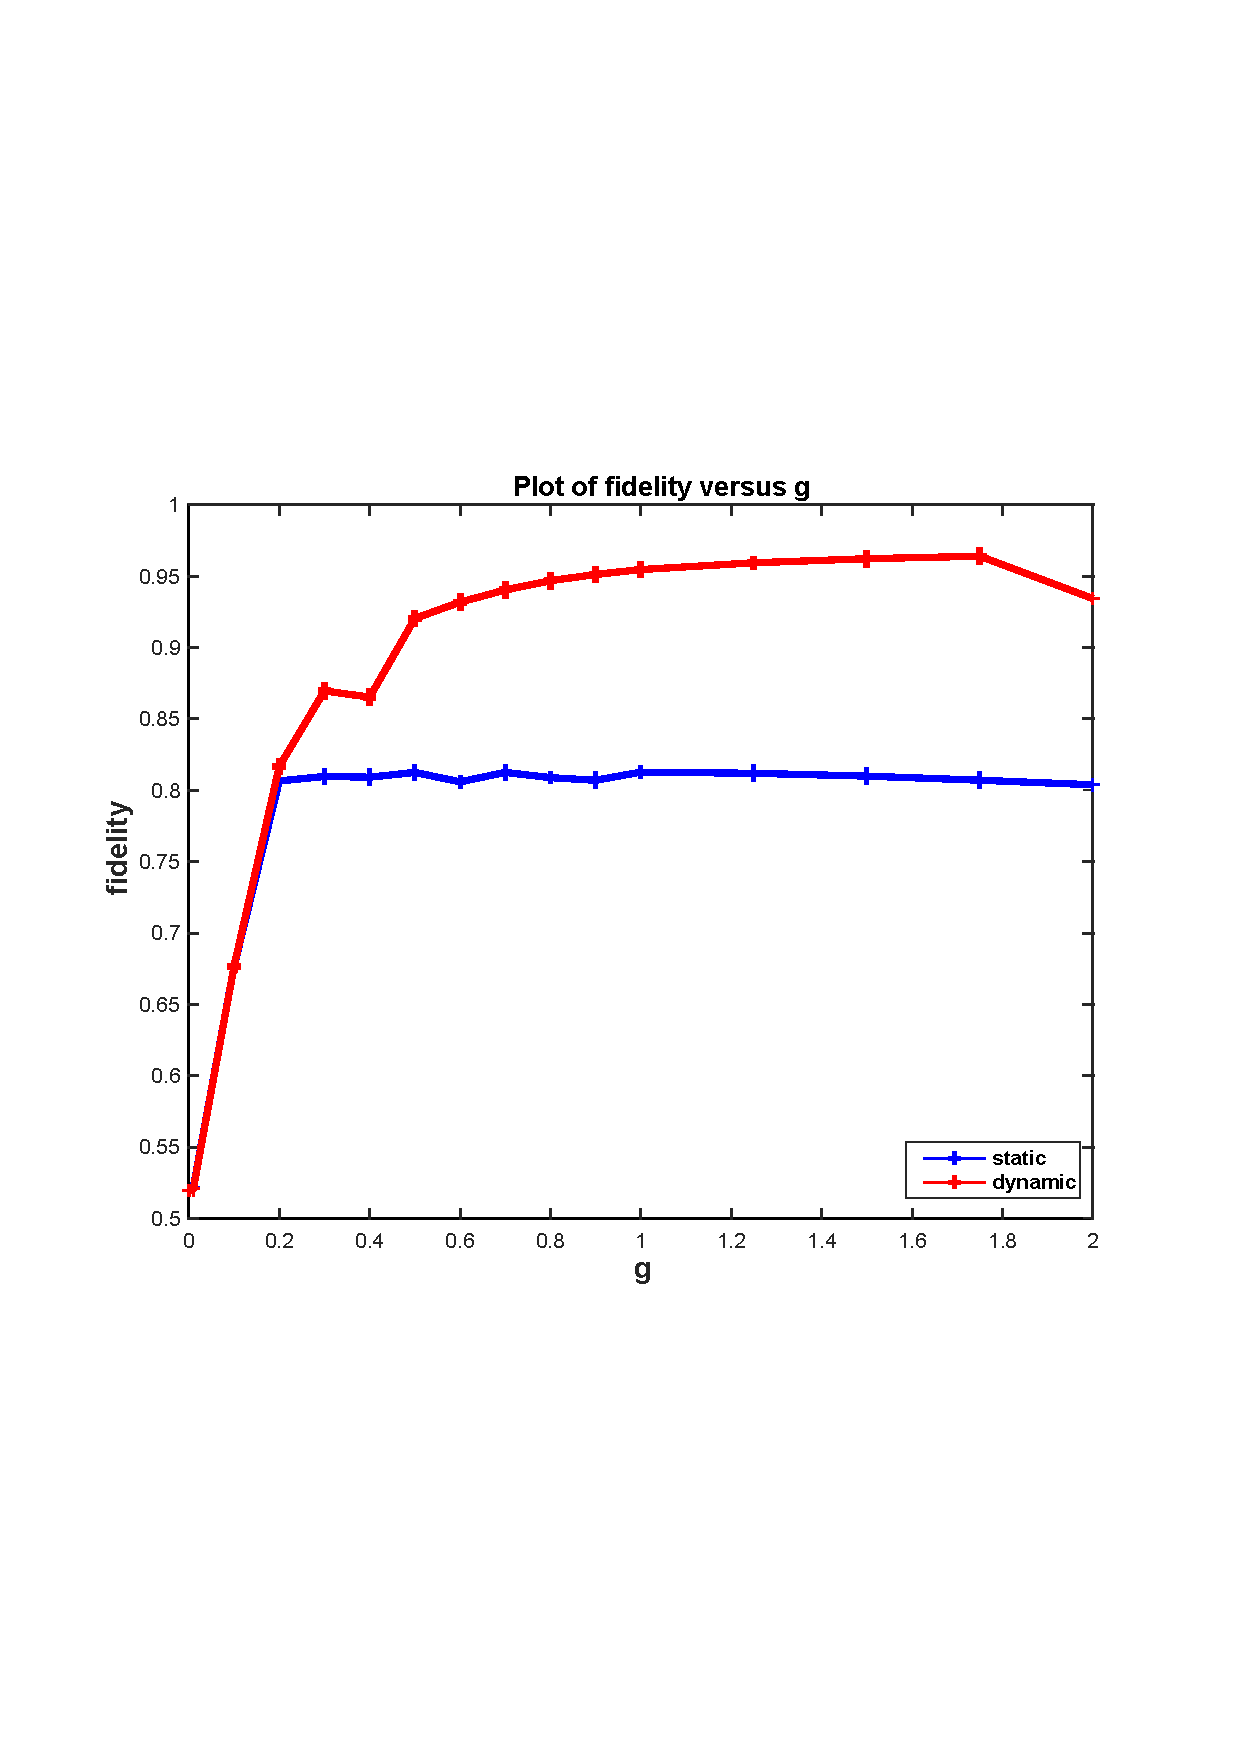
\includegraphics[width=1.1\textwidth]{F_both_in_one}
\caption{Plot of fidelity versus g(coupling strength) for both dynamic as well as static}
\label{F_both_in_one}
\end{figure}
\end{center}
%\lipsum[4-7]


\begin{center}
\begin{figure}%[!h]
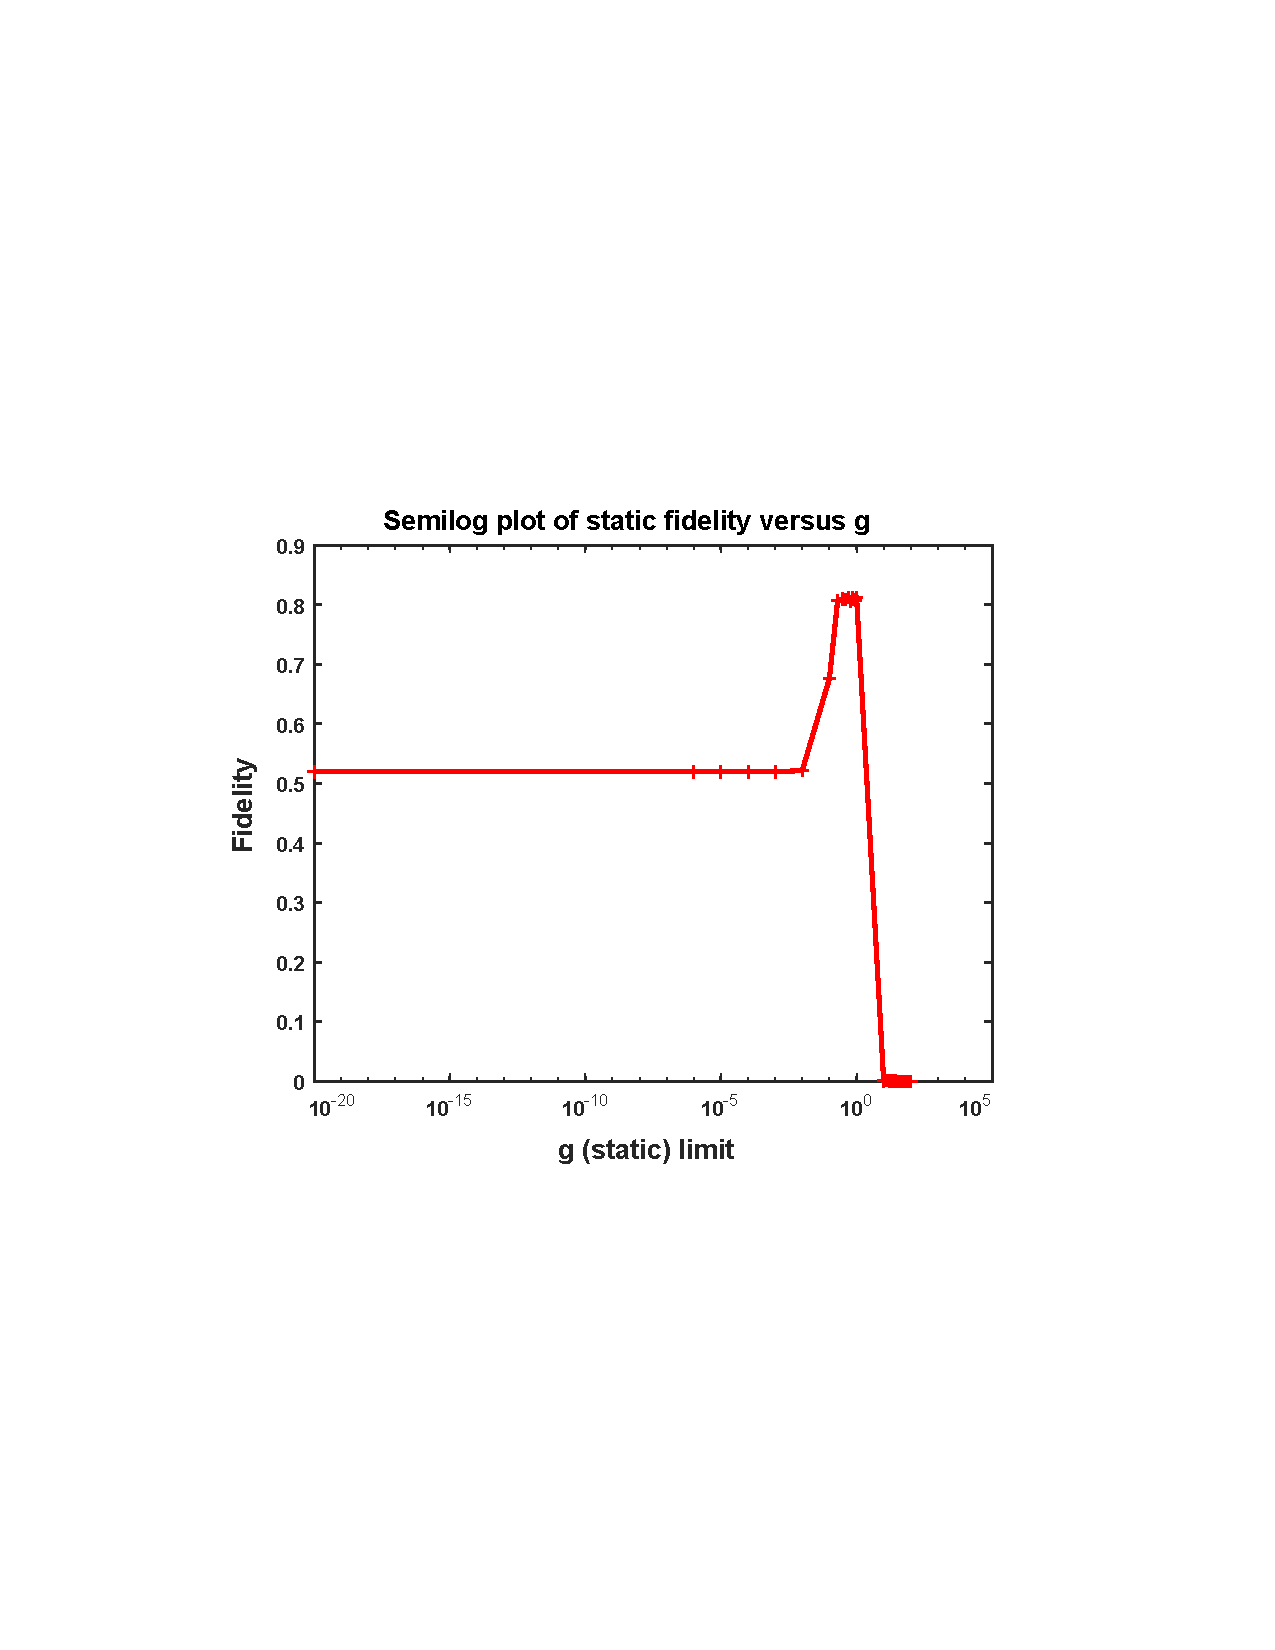
\includegraphics[width=1.1\textwidth]{A_fidelity_static_g__semilog_large_range}
\caption{Semi logarithmic plot of static fidelity versus g(coupling strength). This is plot of the target state fidelity obtained versus the coupling strength. g. For each of the above data points the coupling strength is held at a fixed value for the entire length of the time the system is allowed to evolve. At a time, $t = t_{max}$. we measure the overlap of the target state with the final state in terms of the fidelity metric.}
\label{A_fidelity_static_g__semilog_large_range}
\end{figure}
\end{center}
%\lipsum[4-7]


\begin{center}
\begin{figure}%[!h]
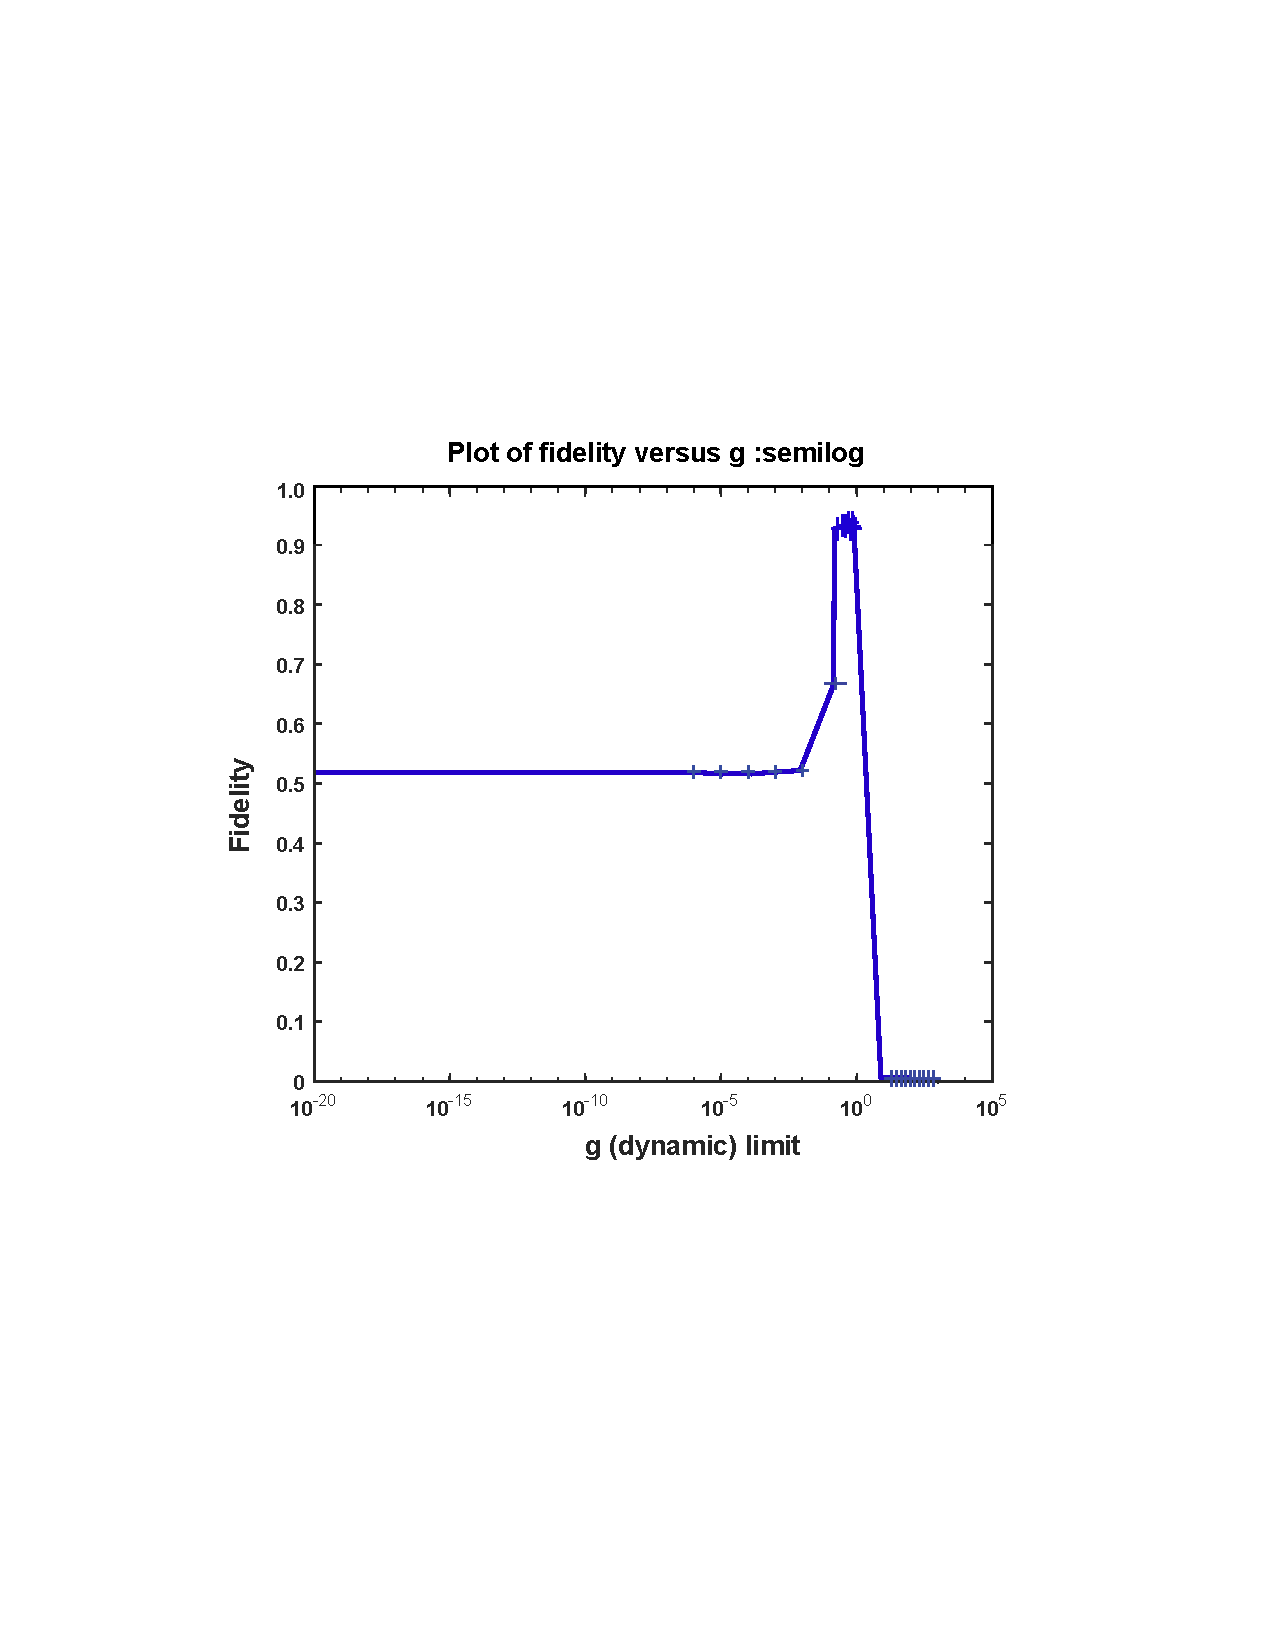
\includegraphics[width=1.1\textwidth]{H-fk_fidelity_static_g__semilog_large_range_-_Final}
\caption{Semi logarithmic plot of dynamic fidelity versus g(coupling strength). This is a plot of the target state fidelity obtained versus the maximum value of the coupling constant $g_{max}$ during the particular run. The coupling strength is varied with time such that the maximum value  in a particular run is less than or equal to $g_{max}$. This is true for all the data points. At time $t=t_{max}$ one measures the over lap of the target state to the state of the system at $t=t_{max}$ in terms of fidelity metric.     }
\label{H-fk_fidelity_static_g__semilog_large_range_-_Final}
\end{figure}
\end{center}
%\lipsum[4-7]

\begin{center}
\begin{figure}%[!h]
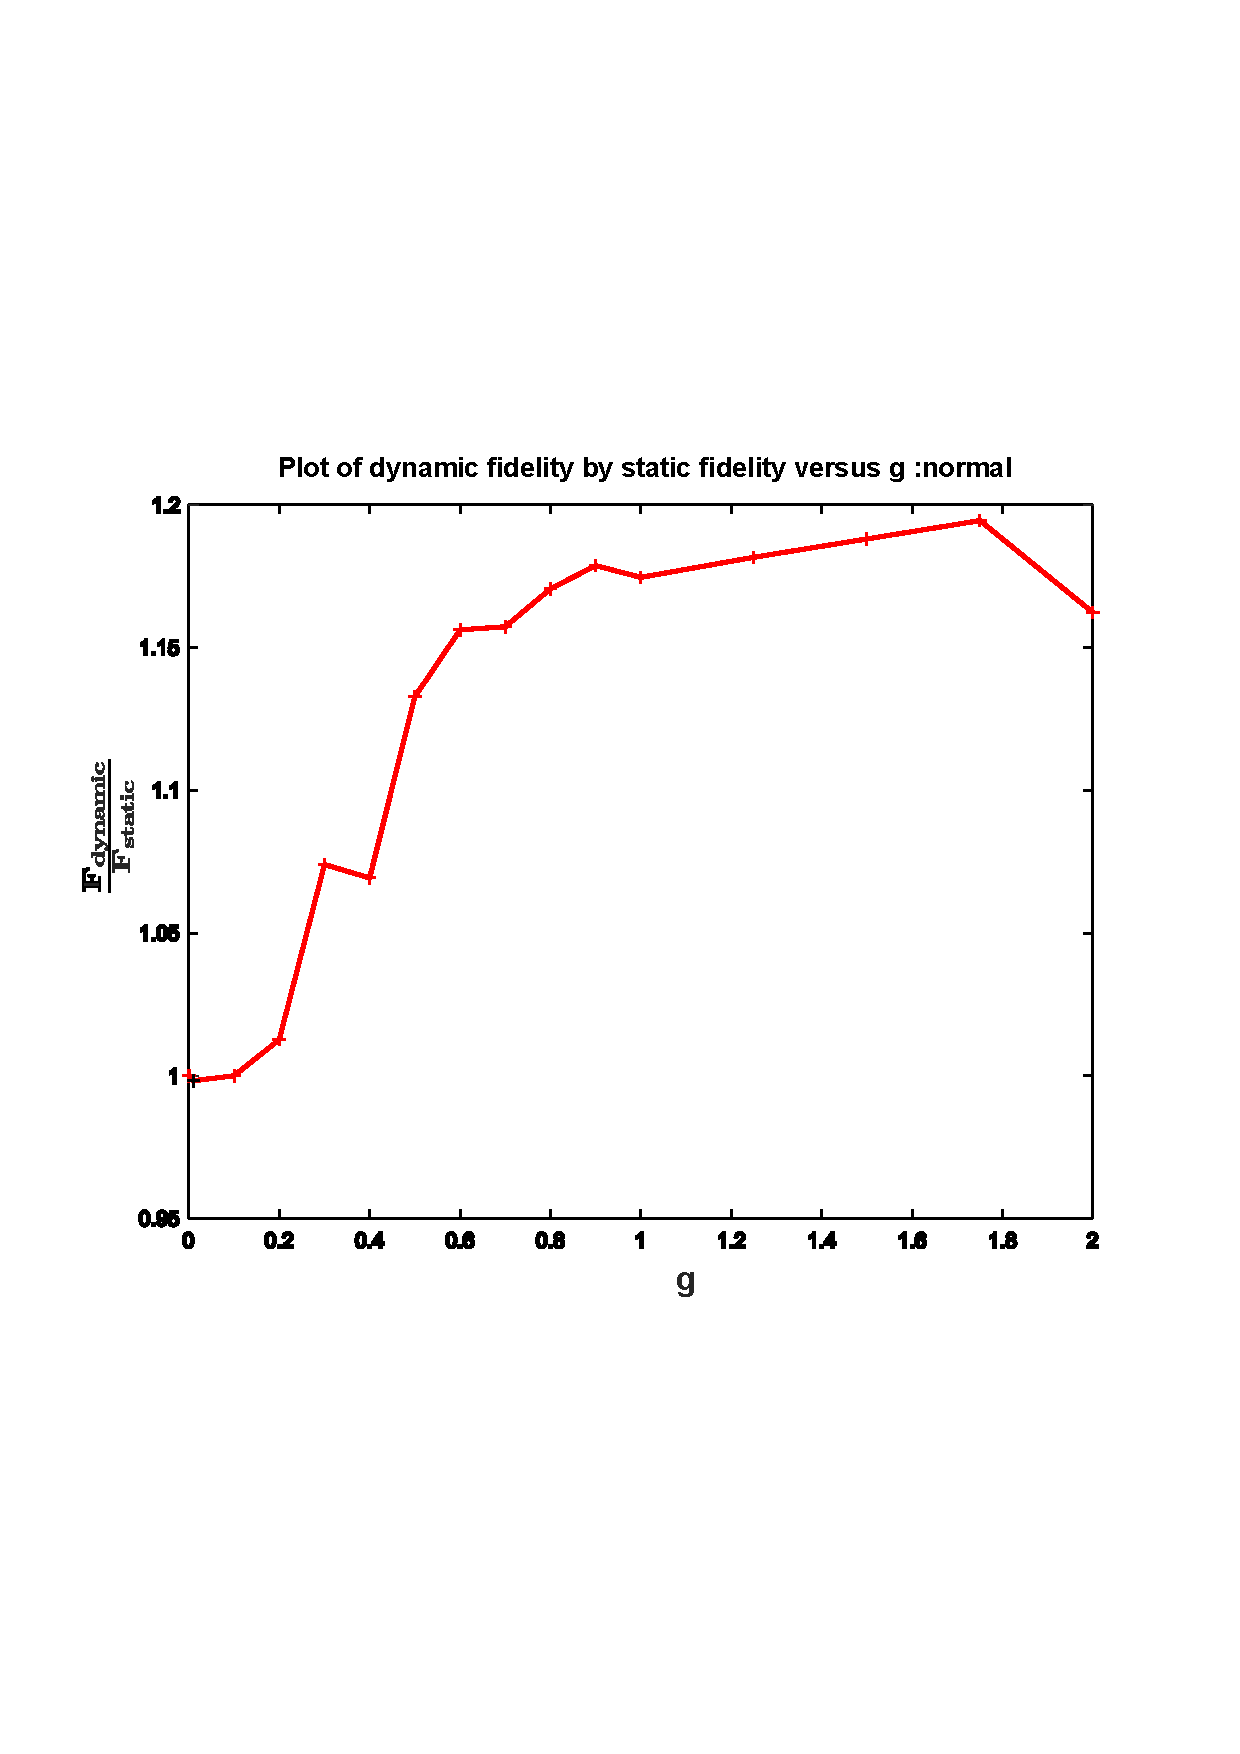
\includegraphics[width=1.1\textwidth]{E_dynamic_static_versus_g__normal}
\caption{Plot of ratio of dynamic fidelity by static fidelity versus g(coupling strength)}
\label{E_dynamic_static_versus_g__normal}
\end{figure}
\end{center}
%\lipsum[4-7]










\begin{comment}
\begin{center}
\begin{figure}%[!h]
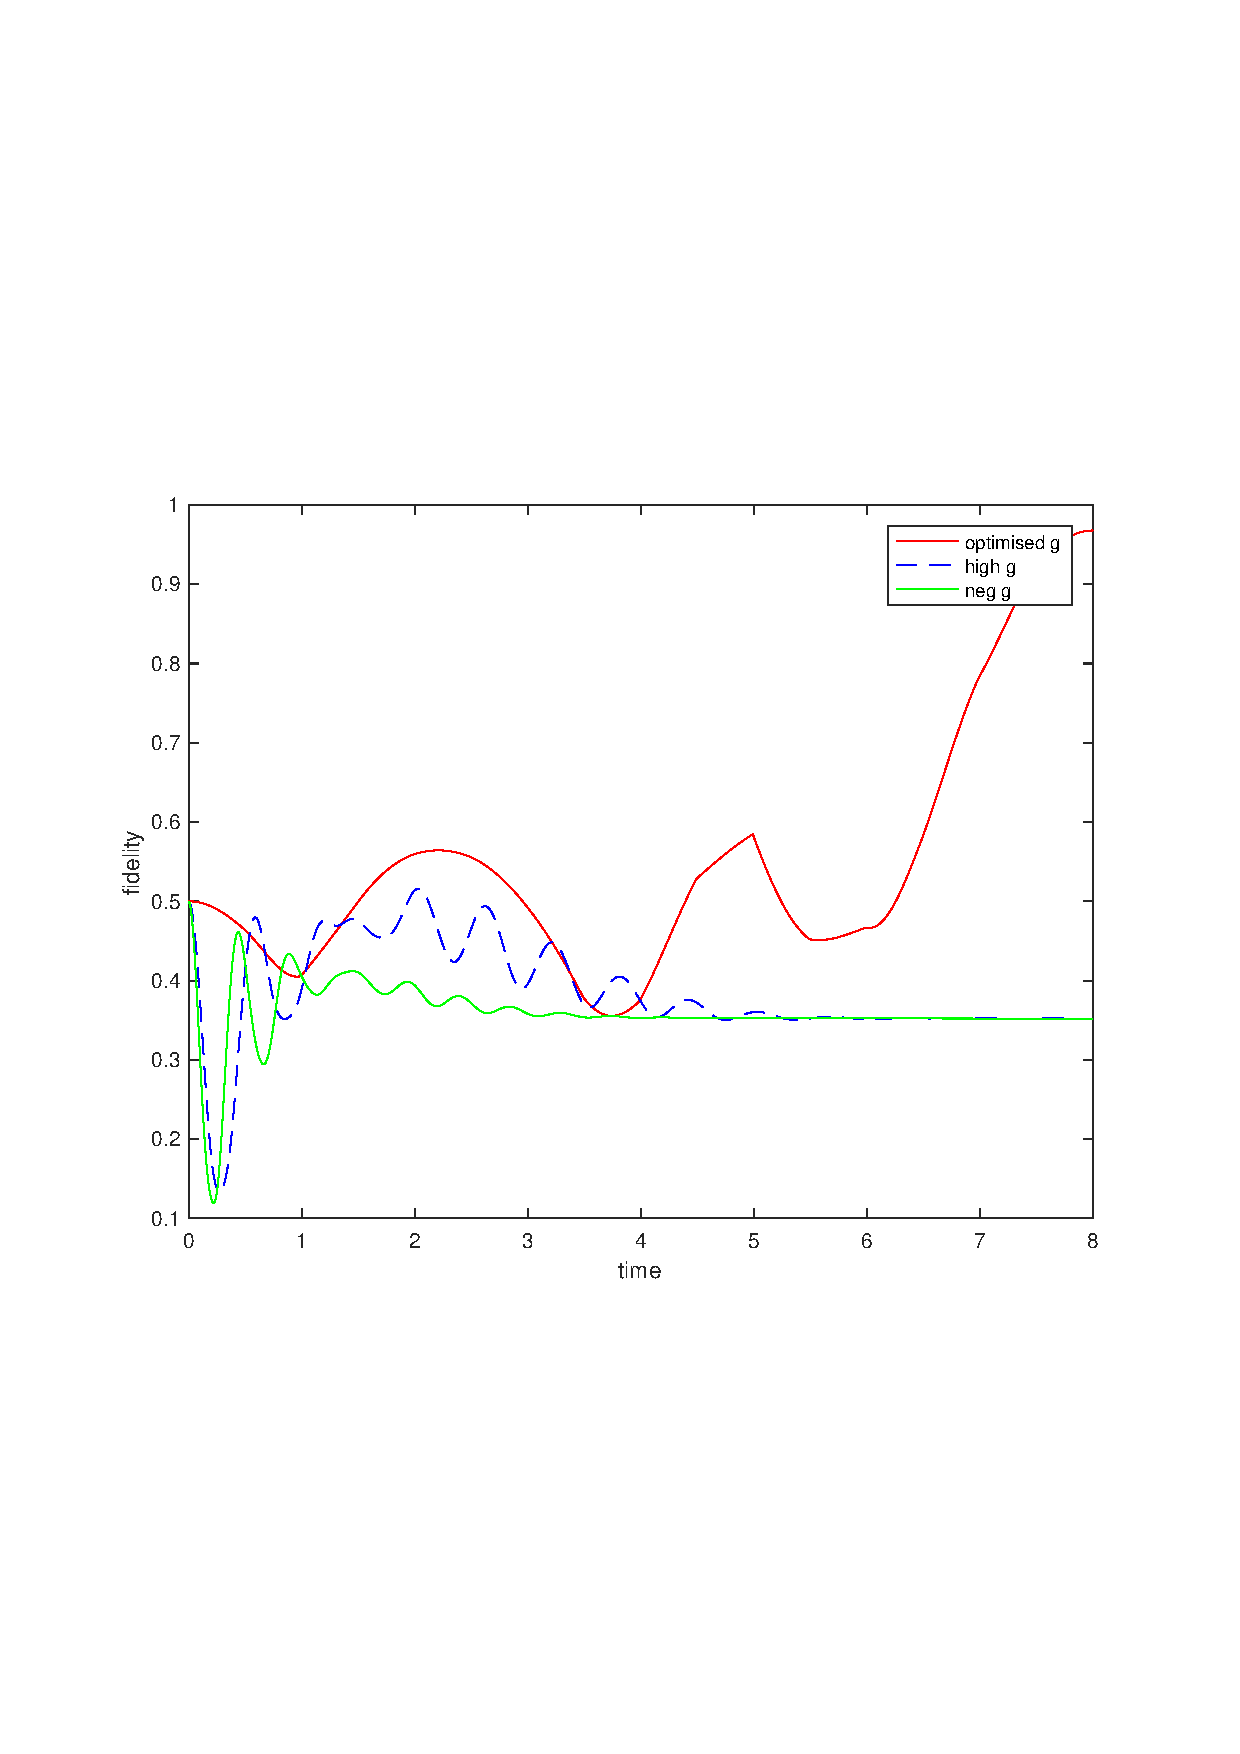
\includegraphics[width=1.0\textwidth]{gvary7}
\caption{Plot of fidelity versus time for different   g (t) }
\label{fig:gvary7}
\end{figure}
\end{center}
%\lipsum[4-7]
\end{comment}













\begin{comment}

\newpage
\begin{center}
\begin{figure}%[!h]
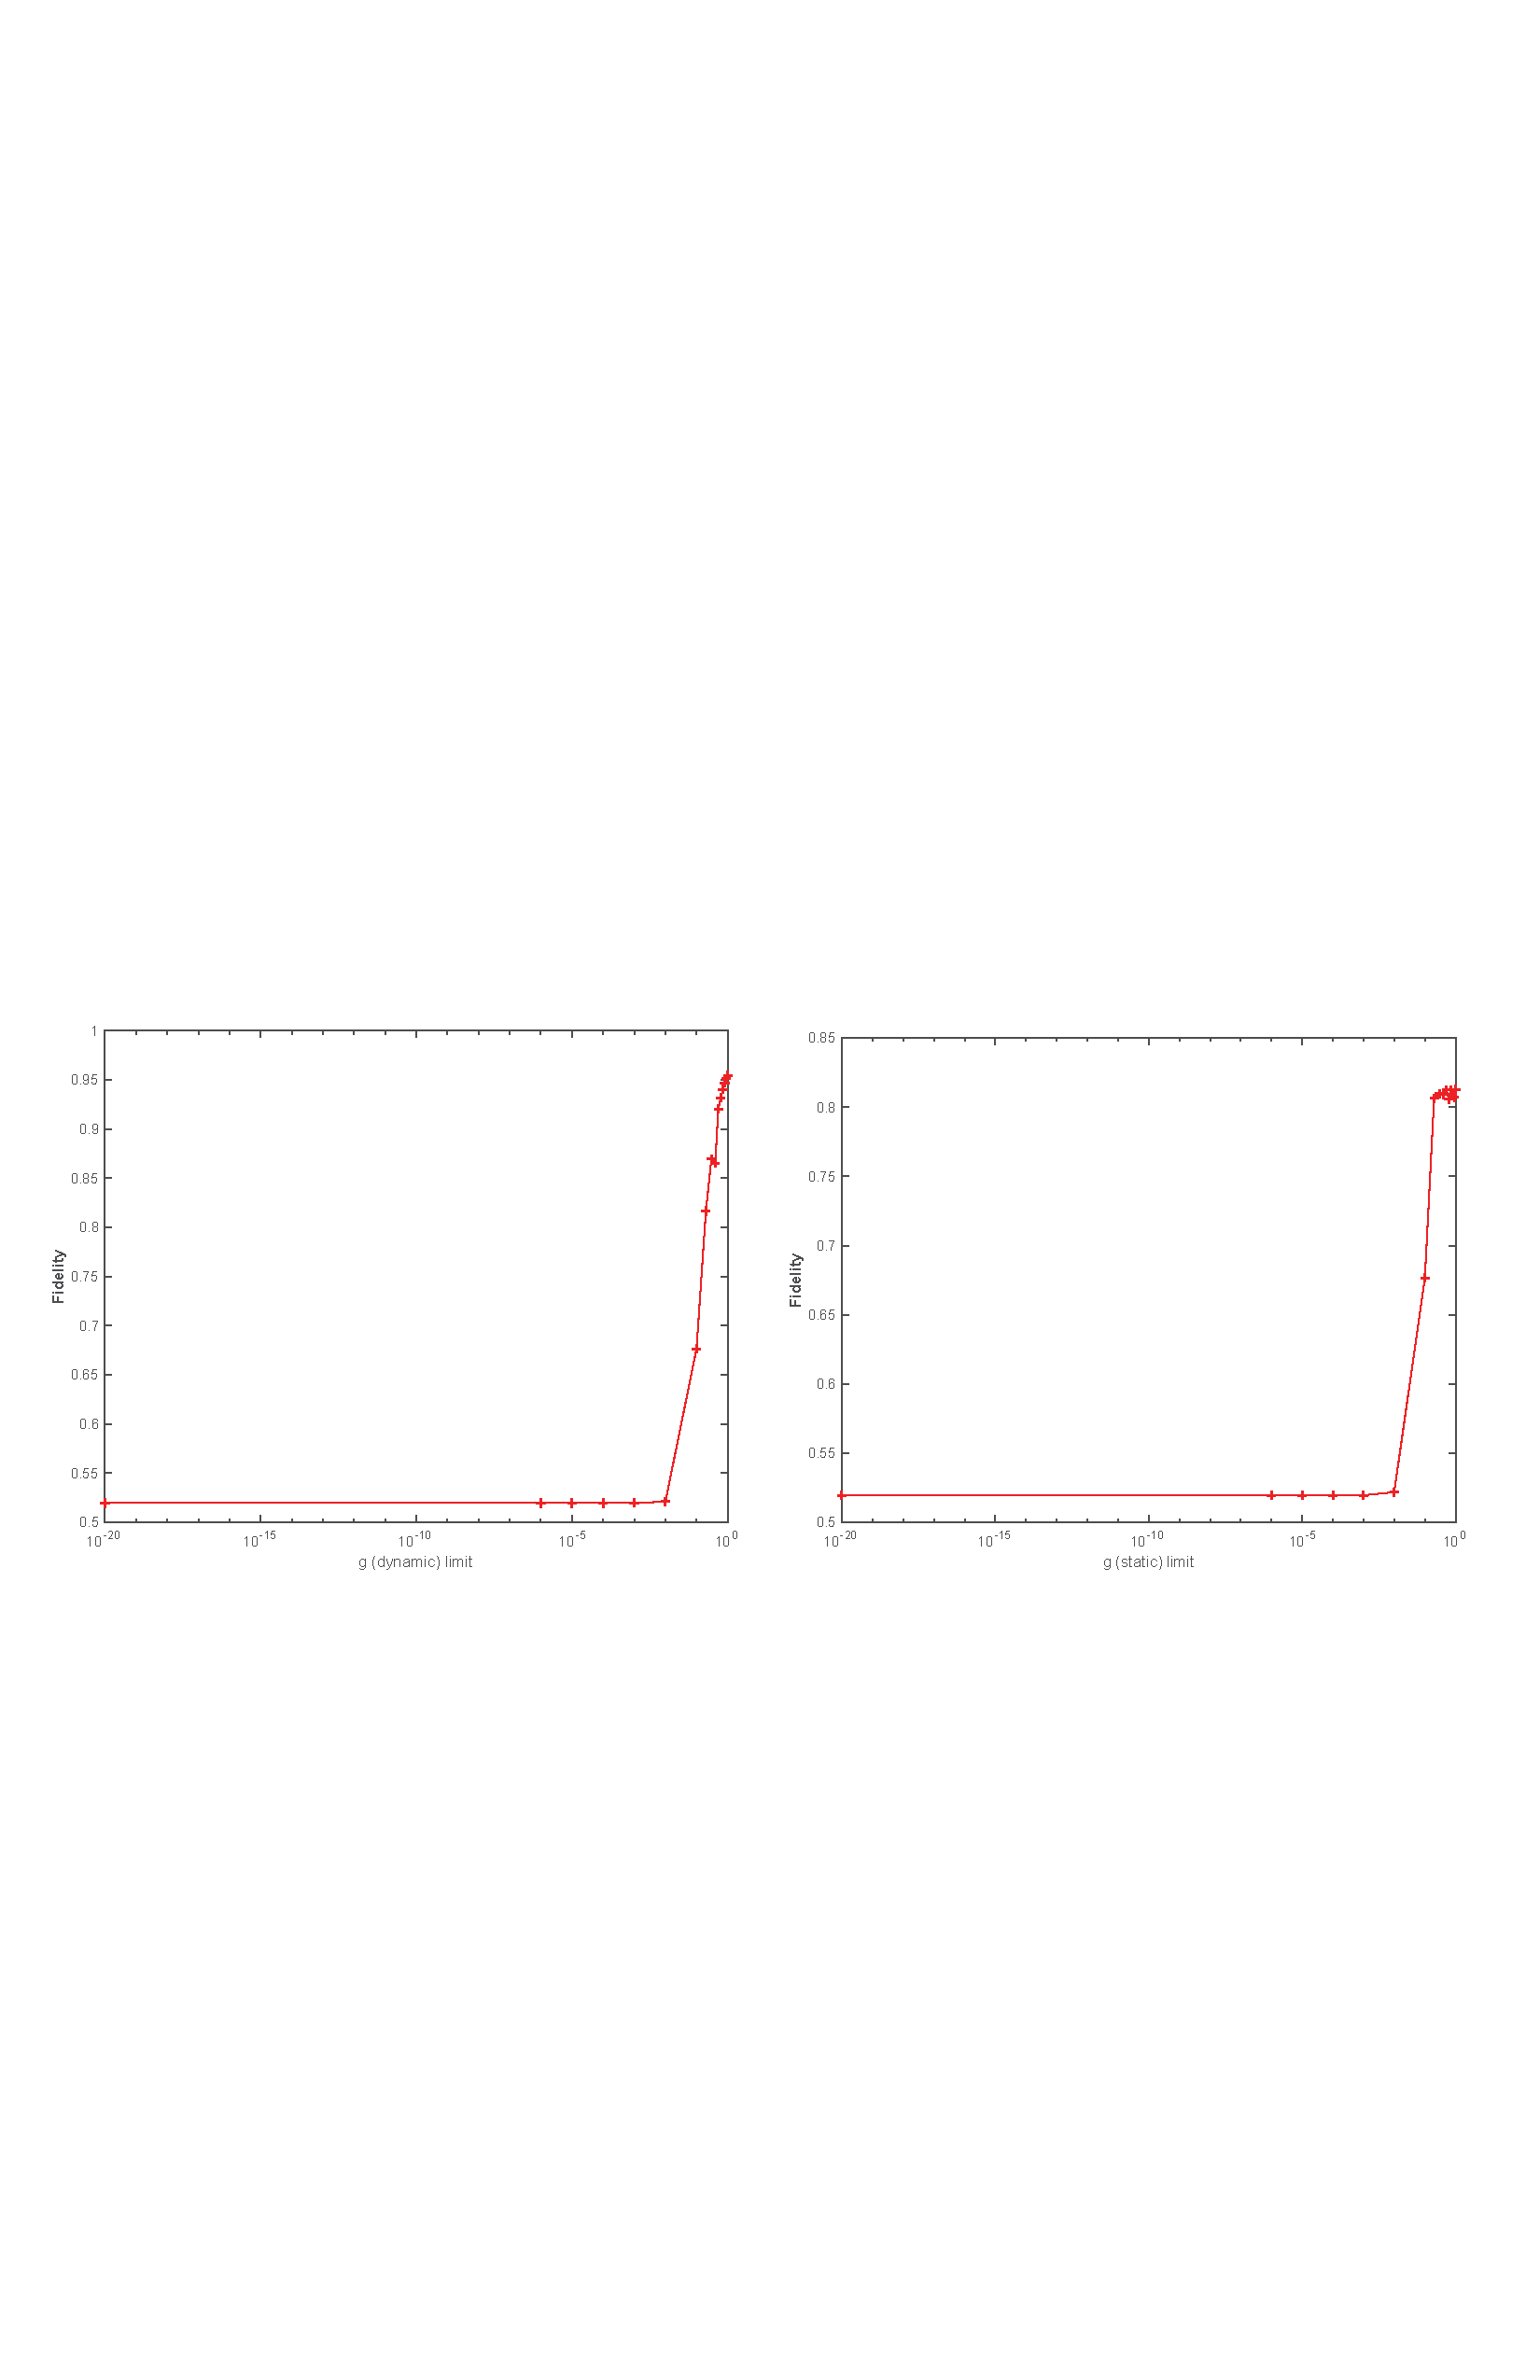
\includegraphics[width=1.1\textwidth]{Integrated_2_graph}
\caption{Semi logarithmic plot of fidelity versus g(coupling strength) for both dynamic as well static. Please note the different scales in Y axis.}
\label{fig:Integrated_2_graph}
\end{figure}
\end{center}
%\lipsum[4-7]





\begin{center}
\begin{figure}%[!h]
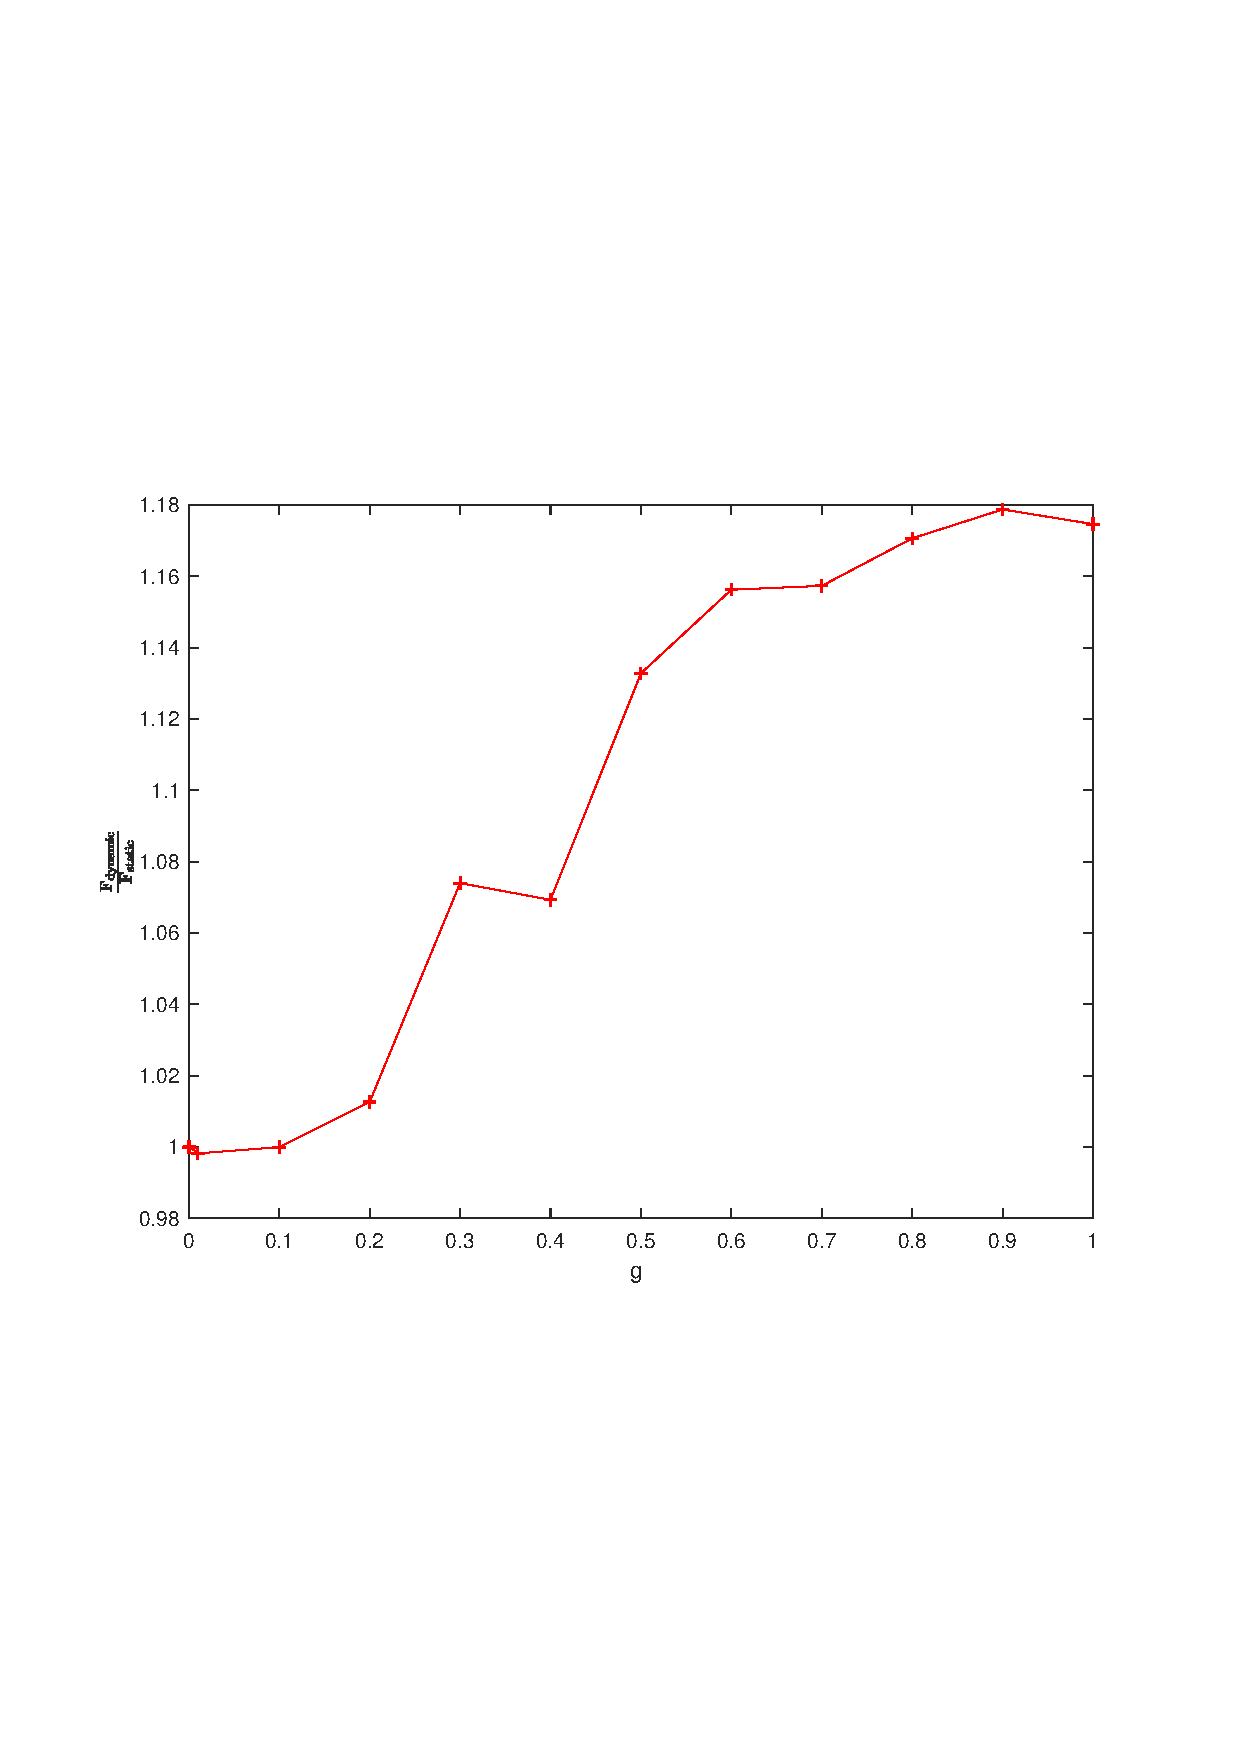
\includegraphics[width=1.0\textwidth]{25-19feb-advantage_normal1}
\caption{Plot of dynamic by static versus g(coupling strength) : normal  }
\label{fig:25-19feb-advantage_normal1}
\end{figure}
\end{center}
%\lipsum[4-7]

\begin{center}
\begin{figure}%[!h]
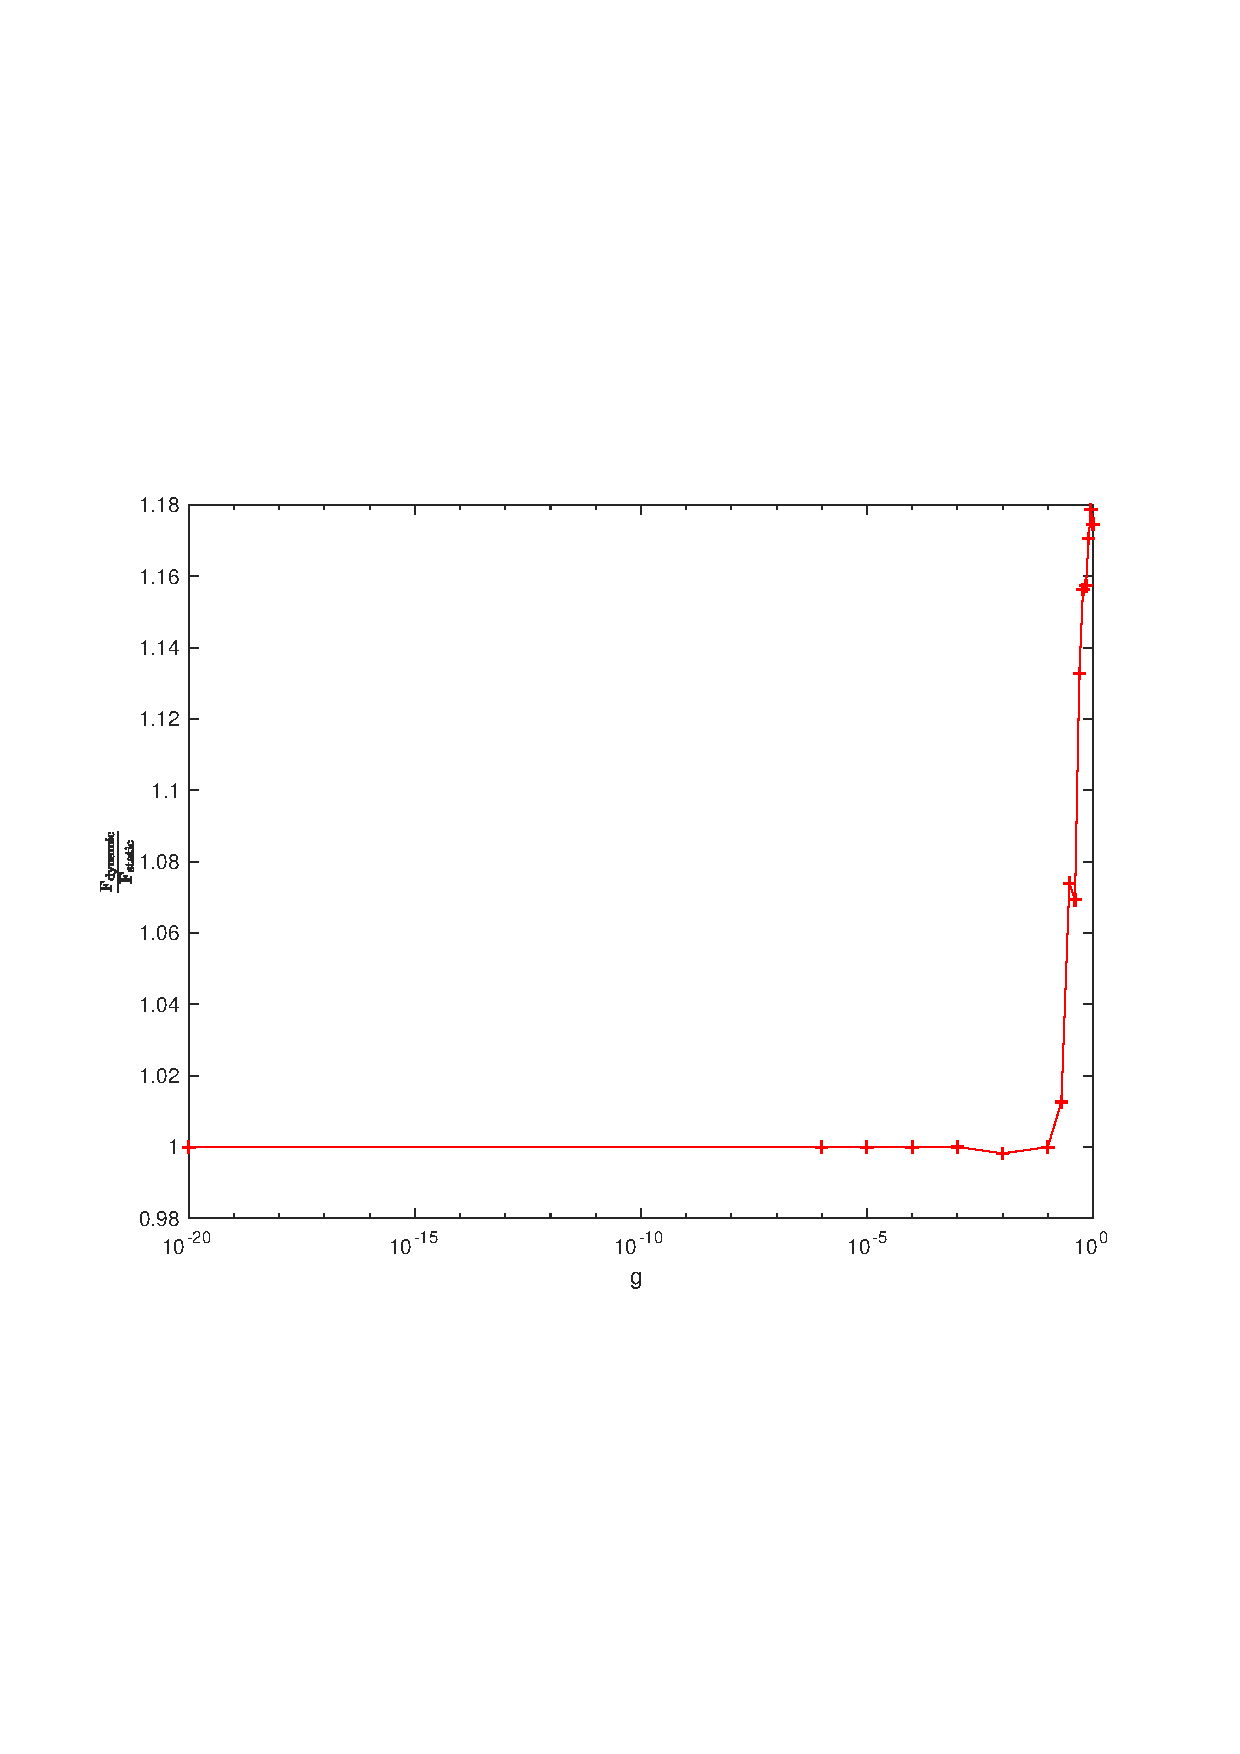
\includegraphics[width=1.0\textwidth]{26-19feb-advantage_semilog}
\caption{Plot of dynamic by static versus g(coupling strength) : semilog }
\label{fig:26-19feb-advantage_semilog}
\end{figure}
\end{center}
%\lipsum[4-7]

\end{comment}
















\begin{comment}



\begin{center}
\begin{figure}%[!h]
\includegraphics[width=1.0\textwidth]{29-19feb-fidelity_dynamic_g__normal}
\caption{Plot of fidelity versus g:normal}
\label{29-19feb-fidelity_dynamic_g__normal}
\end{figure}
\end{center}
%\lipsum[4-7]

\begin{center}
\begin{figure}%[!h]
\includegraphics[width=1.0\textwidth]{30-19feb-fidelity_dynamic_g__semilog}
\caption{Plot of fidelity versus g :semilog}
\label{30-19feb-fidelity_dynamic_g__semilog}
\end{figure}
\end{center}
%\lipsum[4-7]


\begin{center}
\begin{figure}%[!h]
\includegraphics[width=1.0\textwidth]{31-19feb-fidelity_static_g__normal}
\caption{Plot of fidelity versus g :normal   :normal}
\label{31-19feb-fidelity_static_g__normal}
\end{figure}
\end{center}
%\lipsum[4-7]


\begin{center}
\begin{figure}%[!h]
\includegraphics[width=1.0\textwidth]{32-19feb-fidelity_static_g__semilog}
\caption{Plot of fidelity versus g :semilog }
\label{32-19feb-fidelity_static_g__semilog}
\end{figure}
\end{center}
%\lipsum[4-7]


\begin{center}
\begin{figure}%[!h]
\includegraphics[width=1.0\textwidth]{7-fidelity_dynamic_g__normal}
\caption{Plot of fidelity versus g :normal}
\label{7-fidelity_dynamic_g__normal}
\end{figure}
\end{center}
%\lipsum[4-7]


\begin{center}
\begin{figure}%[!h]
\includegraphics[width=1.0\textwidth]{9-fidelity_static_g__normal}
\caption{Plot of fidelity static g :normal  :}
\label{9-fidelity_static_g__normal}
\end{figure}
\end{center}
%\lipsum[4-7]

\end{comment}



\begin{comment}



\begin{center}
\begin{figure}%[!h]
\includegraphics[width=1.0\textwidth]{27-19feb-dynamic_static_versus_g__normal}
\caption{Plot of dynamic by static versus $g$  :normal}
\label{27-19feb-dynamic_static_versus_g__normal}
\end{figure}
\end{center}
%\lipsum[4-7]


\begin{center}
\begin{figure}%[!h]
\includegraphics[width=1.0\textwidth]{28-19feb-dynamic_static_versus_g__semilog}
\caption{Plot of dynamic by static versus $g$ :semilog  }
\label{28-19feb-dynamic_static_versus_g__semilog}
\end{figure}
\end{center}
%\lipsum[4-7]


\begin{center}
\begin{figure}%[!h]
\includegraphics[width=1.0\textwidth]{33-19feb-fidelity_versus_g__normal}
\caption{Plot of fidelity versus g :normal$g$ }
\label{33-19feb-fidelity_versus_g__normal}
\end{figure}
\end{center}
%\lipsum[4-7]




\begin{center}
\begin{figure}%[!h]
\includegraphics[width=1.0\textwidth]{34-19feb-fidelity_versus_g__semilog}
\caption{Plot of fidelity versus $g$:semilog }
\label{34-19feb-fidelity_versus_g__semilogl}
\end{figure}
\end{center}
%\lipsum[4-7]












\begin{figure}
\centering
\includegraphics[width=0.8\textwidth]{1-16feb11.pdf}
\caption{1-16feb11}
\label{fig:1-16feb11}
\end{figure}

\begin{figure}
\centering
\includegraphics[width=0.8\textwidth]{1-16feb11-001.pdf}
\caption{1-16feb11-001}
\label{fig:1-16feb11-001}
\end{figure}


\begin{figure}
\centering
\includegraphics[width=0.8\textwidth]{11-runwith100000.pdf}
\caption{11-runwith100000}
\label{fig:11-runwith100000}
\end{figure}

\begin{figure}
\centering
\includegraphics[width=1.0\textwidth]{5-16feb12.pdf}
\caption{5-16feb12}
\label{fig:5-16feb12}
\end{figure}


\begin{figure}
\centering
\includegraphics[width=1.0\textwidth]{8-16feb6.pdf}
\caption{8-16feb6}
\label{fig:8-16feb6}
\end{figure}

\begin{figure}
\centering
\includegraphics[width=1.0\textwidth]{2-16feb15.pdf}
\caption{2-16feb15}
\label{fig:2-16feb15}
\end{figure}

\begin{figure}
\centering
\includegraphics[width=1.0\textwidth]{3-16feb16.pdf}
\caption{3-16feb16}
\label{fig:3-16feb16}
\end{figure}
\lipsum[1-3]
\end{comment}







